
%!TEX ROOT=ctutest.tex

\chapter{Identifikované parametry}

Postupem popsaným v sekci \ref{postup_identifikace_ch} se podařilo identifikovat všechny neznámé parametry. Identifikované parametry jsou uvedeny v tabulce \ref{tab_ind_hodnot}. V následující tabulce \ref{tab_ind_hodnot_3d} jsou pro srovnání vypsané hodnoty identifikované z 3D modelu robota (viz sekce \ref{z_3d_modelu_sec}). Hodnoty v tabulkách jsou uvedeny v základních jednotkách SI. 
\\
\begin{table}[htbp]
  \centering
  \caption{Tabulka identifikovaným parametrů z rovnic}
    \begin{tabular}{c|cccccccccc}
    \multicolumn{1}{c|}{Osa} & \multicolumn{1}{c}{$I_{xx}$} & \multicolumn{1}{c}{$I_{yy}$} & \multicolumn{1}{c}{$I_{zz}$} & \multicolumn{1}{c}{$d_x$} & \multicolumn{1}{c}{$d_y$} & \multicolumn{1}{c}{$d_z$} & \multicolumn{1}{c}{$m$} & \multicolumn{1}{c}{$f_v$} & \multicolumn{1}{c}{$f_c$} \\
    \hline
    1  & 0     & 0     & 3.963 & 0     & 0     & 0     & 0     & 93.540 &  6.473 \\
    2  & 0.197 & 3.078 & 1.967 & 0.301 & 0.034 & 0     & 19.30 & 93.240 & 21.107 \\
    3  & 0.490 & 3.025 & 0.799 &-0.038 &-0.133 &-0.006 & 26.47 & 24.510 &  2.486 \\
    4  & 1.737 & 0.509 & 0.637 &-0.037 & 0.024 &-0.027 & 7.41  &  7.235 &  1.594 \\
    5  & 0.105 & 0.353 & 0.218 & 0.030 & 0     &-0.140 & 2.53  &  1.863 &  1.033 \\
    6  & 0.179 & 0.206 & 0.027 & 0     & 0     & 0.133 & 0.60  &  1.148 &  0.396 \\
    \end{tabular}%
  \label{tab_ind_hodnot}%
\end{table}%

\begin{table}[htbp]
  \centering
  \caption{Tabulka identifikovaným parametrů z 3D modelu}
    \begin{tabular}{c|cccccccccc}
    \multicolumn{1}{c|}{Osa} & \multicolumn{1}{c}{$I_{xx}$} & \multicolumn{1}{c}{$I_{yy}$} & \multicolumn{1}{c}{$I_{zz}$} & \multicolumn{1}{c}{$d_x$} & \multicolumn{1}{c}{$d_y$} & \multicolumn{1}{c}{$d_z$} & \multicolumn{1}{c}{$m$} & \multicolumn{1}{c}{$f_v$} & \multicolumn{1}{c}{$f_c$} \\
    \hline
    1  & 0.322   & 0.467   & 0.478   & 0.091 & 0.067 & 0.006 & 26.98 & - & - \\
    2  & 0.541   & 0.552   & 0.044   & 0.333 & 0.002 & 0.039 & 15.92 & - & - \\
    3  & 0.775   & 0.750   & 0.210   &-0.032 &-0.008 &-0.034 & 25.85 & - & - \\
    4  & 0.010   & 0.020   & 0.024   & 0     & 0.109 &-0.008 & 4.09  & - & - \\
    5  & 0.002   & 0.004   & 0.004   & 0     &-0.01  & 0     & 1.62  & - & - \\
    6  & 0.00006 & 0.00003 & 0.00003 & 0     & 0     & 0.111 & 0.02  & - & - \\
    \end{tabular}%
  \label{tab_ind_hodnot_3d}%
\end{table}%

Porovnáním hodnot v obou tabulkách je patrné, že se většina parametrů, snad jen s výjimkou hmotností ramen, poměrně výrazně liší. Dalším rozdílem je, že z 3D modelu není možné získat informace o koeficientech tření v jednotlivých osách, zatímco odvození z rovnic s třením počítá. Jak bude patrné ze simulace odvozených parametrů, tření má na dynamiku nezanedbatelný vliv.

\section{Simulace odvozených parametrů}

Na následujících obrázcích jsou odsimulované točivé momenty s odvozenými parametry pro osy 4 až 6. Pro další osy simulace provedeny nebyly, protože se pro ně nepodařilo správně odvodit všechny jejich dynamické parametry.

Na obrázku \ref{osa6_prub_a} je porovnání mezi skutečným naměřeným momentem a vypočítaným z odvozených parametrů pro osu 6. Na druhém obrázku \ref{osa6_prub_b} je poté zobrazena okamžitá a průměrná odchylka mezi naměřeným a vypočítaným momentem. 

\begin{figure}[!h]
  \centering
  \subfloat[Srovnání naměřených a vypočítaných momentů]{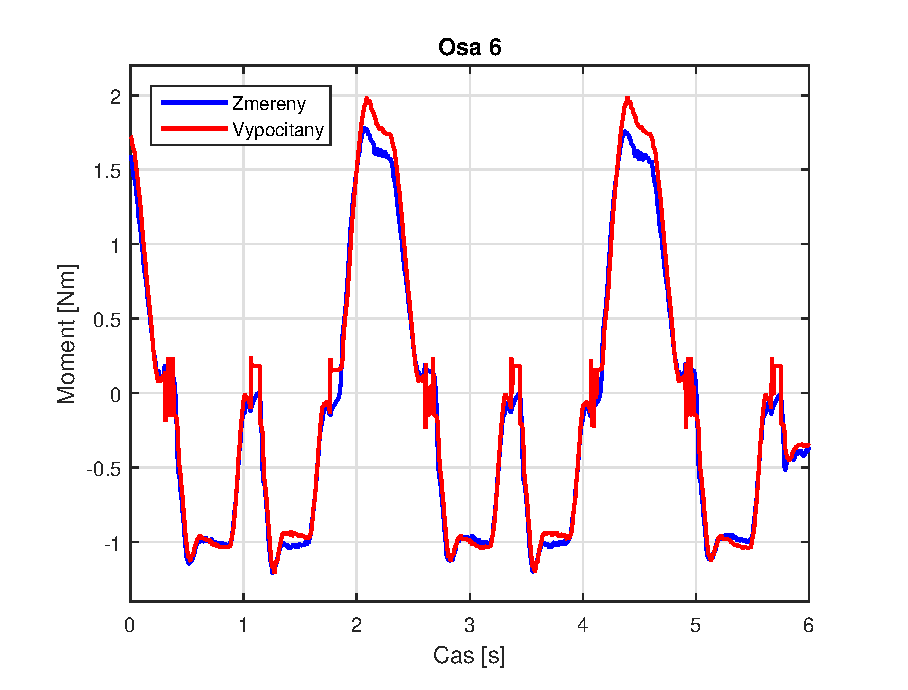
\includegraphics[width=0.6\textwidth]{Osa_6}\label{osa6_prub_a}}
  \hfill
  \subfloat[Okamžitá a průměrná odchylka]{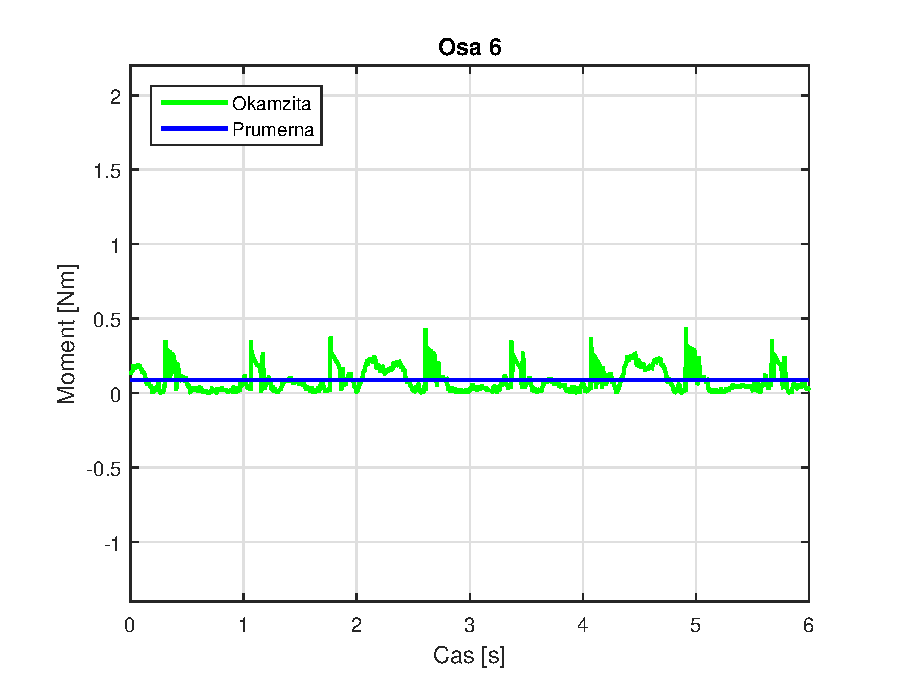
\includegraphics[width=0.5\textwidth]{Osa_6_odch}\label{osa6_prub_b}}
  \caption{Točivé momenty pro osu 6.}
  \label{osa6_prub}
\end{figure}

Stejné průběhy pro osu 5 jsou na obrázku \ref{osa5_prub} a pro osu 4 na obr. \ref{osa4_prub}.

\begin{figure}[!h]
  \centering
  \subfloat[Srovnání naměřených a vypočítaných momentů]{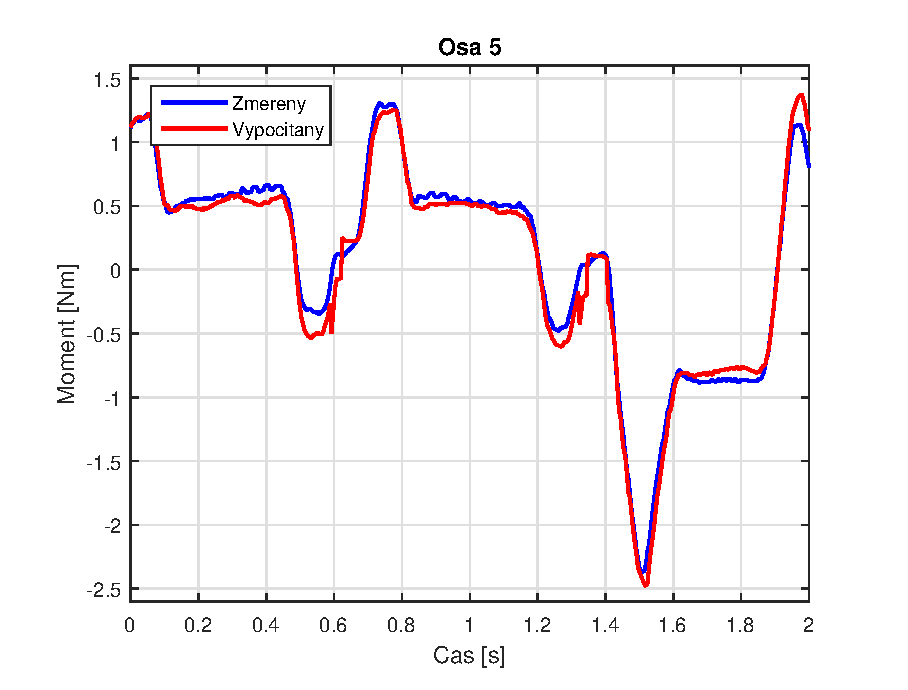
\includegraphics[width=0.5\textwidth]{Osa_5}\label{osa5_prub_a}}
  \hfill
  \subfloat[Okamžitá a průměrná odchylka]{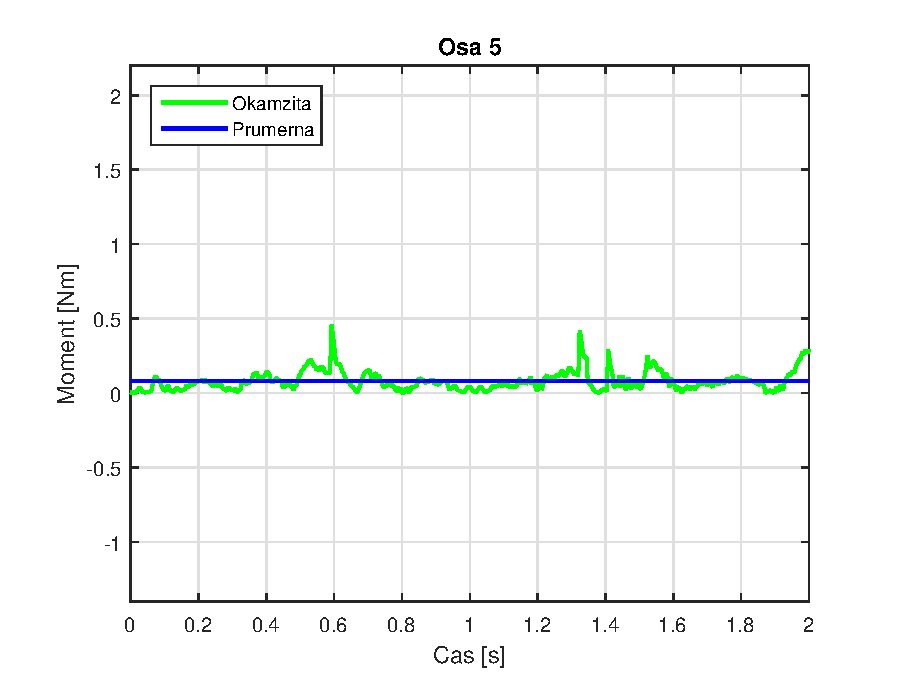
\includegraphics[width=0.5\textwidth]{Osa_5_odch}\label{osa5_prub_b}}
  \caption{Točivé momenty pro osu 5.}
  \label{osa5_prub}
\end{figure}
\newpage

\begin{figure}[!h]
  \centering
  \subfloat[Srovnání naměřených a vypočítaných momentů]{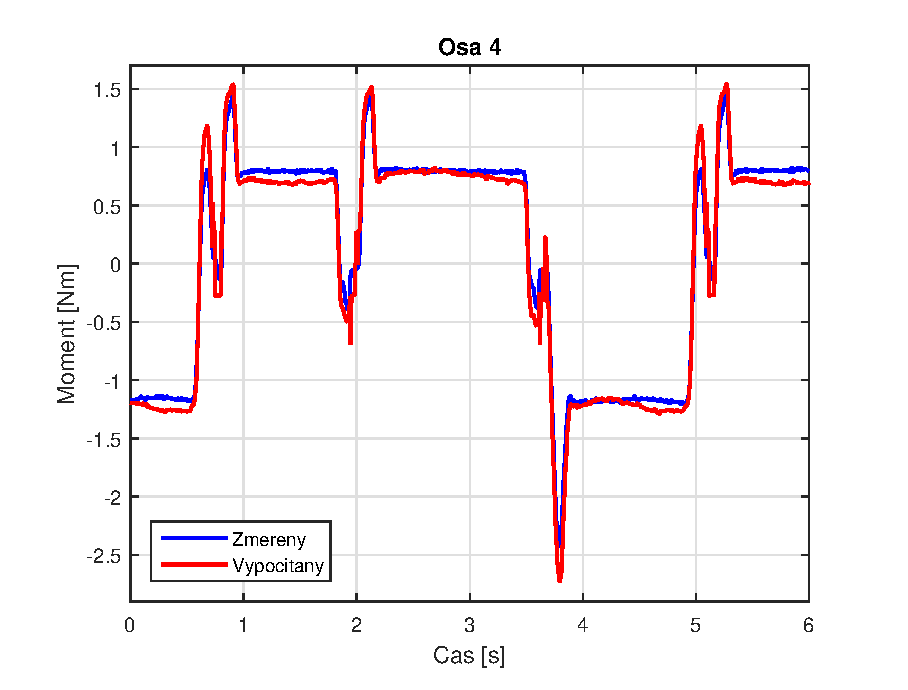
\includegraphics[width=0.5\textwidth]{Osa_4}\label{osa4_prub_a}}
  \hfill
  \subfloat[Okamžitá a průměrná odchylka]{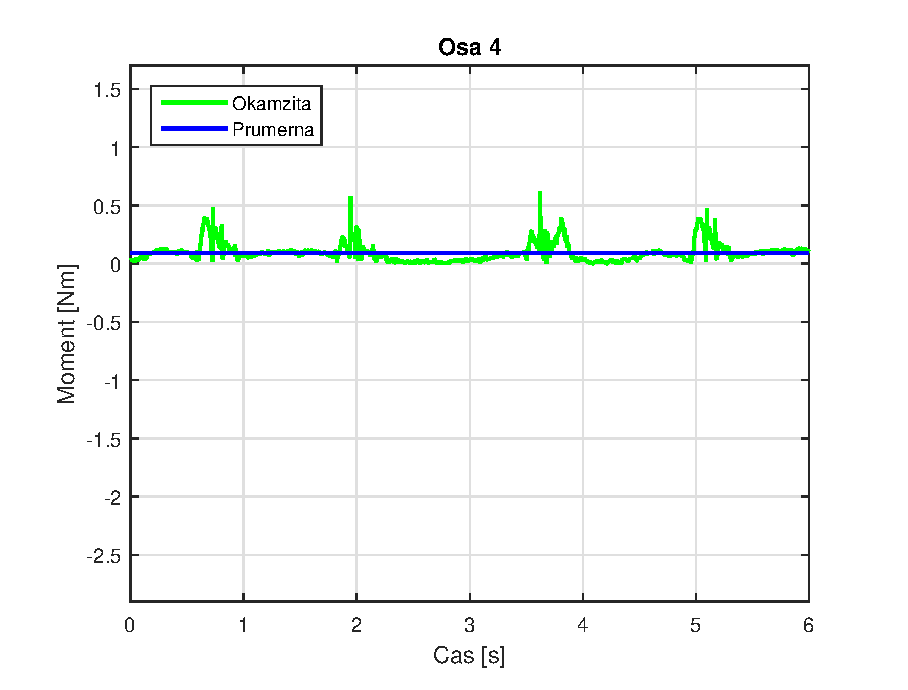
\includegraphics[width=0.5\textwidth]{Osa_4_odch}\label{osa4_prub_b}}
  \caption{Točivé momenty pro osu 4.}
  \label{osa4_prub}
\end{figure}

Z výše uvedených průběhů je patrné, že vypočítané a naměření průběhy si poměrně odpovídají. Ve všech případech se průměrná odchylka pohybuje kolem jedné desetiny Nm a maximální okamžitá odchylka nepřesahuje šest desetin Nm. 

 